\documentclass{bredelebeamer}

%%%%%%%%%%%%%%%%%%%%%%%%%%%%%%%%%%%%%%%%%%%%%%%%

\title[Programación en MatLAB]{Introducción a la programación con MatLAB}
\subtitle{Módulo 03 - Funciones internas de matlab}

\author{Autor1 - Autor2 - Autor3\inst{1}}
\institute[UTN.BA]
{
  \inst{1}%
  Universidad Tecnológica Nacional\\
  Facultad Regional Buenos Aires
  }

\date{día agosto 2018}

\subject{Taller de programación}

\logo{

\includegraphics[scale=0.15]{images/logo.png}
}

%%%%%%%%%%%%%%%%%%%%%%%%%%%%%%%%%%%%%%%%%%%%%%%%%%%%%%%%%%%%%%%%%%%%%
\begin{document}

\begin{frame}
  \titlepage 
\end{frame}

%%%%%%%%%%%%%%%%%%%%%%%%%%%%%%%%%%%%%%%%%%%%%%%%%%%%%%%%%%%%%%%%%%%%%

% Sección de funciones de matlab

%%%%%%%%%%%%%%%%%%%%%%%%%%%%%%%%%%%%%%%%%%%%%%%%%%%%%%%%%%%%%%%%%%%%%

\section{Funciones internas de Matlab}

\begin{frame}{Funciones matemáticas elementales}
\begin{table}[]
\centering
\begin{tabular}{|c|c|}
\hline
Función  & Significado                       \\ \hline
abs(x)   & Encuentra el valor absoluto de x  \\ \hline
sqrt(x)  & Encuentra la raíz cuadrada de x   \\ \hline
los(x)   & Calcula el logaritmo natural de x \\ \hline
log10(x) & Calcula el logaritmo base 10 de x \\ \hline
\end{tabular}
\end{table}
\end{frame}

\begin{frame}{Funciones de redondeo}
\begin{table}[]
\centering
\begin{tabular}{|c|c|}
\hline
Función  & Significado                                              \\ \hline
round(x) & Redondea x al entero más cercano                         \\ \hline
fix(x)   & Redondea x al entero más cercano a cero                  \\ \hline
floor(x) & Redondea x al entero más cercano hacia infinito negativo \\ \hline
ceil(x)  & Redondea x al entero más cercano hacia infinito positivo \\ \hline
\end{tabular}
\end{table}
\end{frame}

\begin{frame}{Funciones trigonométricas}
\begin{table}[]
\centering
\begin{tabular}{|c|c|}
\hline
Función & Significado                                   \\ \hline
sin(x)  & Seno de x cuando x se expresa en radianes     \\ \hline
cos(x)  & Coseno de x cuando x se expresa en radianes   \\ \hline
tan(x)  & Tangente de x cuando x se expresa en radianes \\ \hline
asin(x) & Arcoseno de x                                 \\ \hline
sinh(x) & Seno hiperbólico de x                         \\ \hline
\end{tabular}
\end{table}
\end{frame}

\begin{frame}{Funciones estadísticas}
\begin{table}[]
\centering
\begin{tabular}{|c|c|}
\hline
Función   & Significado                                            \\ \hline
mean(x)   & Calcula el valor medio de los elementos de un vector x \\ \hline
median(x) & Calcula la mediana de los elementos de un vector x     \\ \hline
\end{tabular}
\end{table}
\end{frame}

\begin{frame}{Ejercicio práctico 2}
Considere la siguiente matriz:
\begin{equation*}
x = [4 90 85 75 ; 2 55 65 75 ; 3 78 82 79 ; 1 84 92 93]
\end{equation*}
\begin{enumerate}
\item Cuál es el valor medio en cada columna?
\item Cuál es la mediana para cada columna?
\item Cuál es el valor medio en cada fila?
\item Cuál es la mediana para cada fila?
\item Cuál es la mediana para toda la matriz?
\end{enumerate}
\end{frame}

\begin{frame}{Máximos y mínimos}
Máximos y mínimos en vectores
\begin{table}[]
\centering
\begin{tabular}{|c|c|}
\hline
max(x)             & Encuentra el valor más grande en un vector x                                                                           \\ \hline
min(x)             & Encuentra el valor mas pequeño en un vector x                                                                          \\ \hline
{[}a,b{]} = max(x) & \begin{tabular}[c]{@{}c@{}}Encuentra el valor más grande en un vector x \\ y su ubicación en el vector x\end{tabular}  \\ \hline
{[}a,b{]} = min(x) & \begin{tabular}[c]{@{}c@{}}Encuentra el valor mas pequeño en un vector x \\ y su ubicación en el vector x\end{tabular} \\ \hline
\end{tabular}
\end{table}
\begin{alertblock}{Tener en cuenta}
Todas las funciones en esta sección funcionan sobre las columnas en matrices bidimensionales. Si su análisis de datos requiere que evalúe datos en filas, los datos se deben transponer.
\end{alertblock}
\end{frame}

\begin{frame}{Máximos y mínimos}
Máximos y mínimos en matrices
\begin{table}[]
\centering
\begin{tabular}{|c|c|}
\hline
max(x)             & \begin{tabular}[c]{@{}c@{}}Crea un vector fila que contiene el elemento máximo de cada columna \\ de una matriz x\end{tabular}                                                                                         \\ \hline
min(x)             & \begin{tabular}[c]{@{}c@{}}Crea un vector fila que contiene el elemento mínimo de cada columna \\ de una matriz x\end{tabular}                                                                                         \\ \hline
{[}a,b{]} = max(x) & \begin{tabular}[c]{@{}c@{}}Crea un vector fila que contiene el elemento máximo de cada columna \\ de una matriz x  y regresa un vector fila con la ubicación \\ del máximo en cada columna de la matriz x\end{tabular} \\ \hline
{[}a,b{]} = min(x) & \begin{tabular}[c]{@{}c@{}}Crea un vector fila que contiene el elemento mínimo de cada columna \\ de una matriz x y regresa un vector fila con la ubicación \\ del mínimo en cada columna de la matriz x\end{tabular}  \\ \hline
\end{tabular}
\end{table}
\begin{alertblock}{Tener en cuenta}
Todas las funciones en esta sección funcionan sobre las columnas en matrices bidimensionales. Si su análisis de datos requiere que evalúe datos en filas, los datos se deben transponer.
\end{alertblock}
\end{frame}

\begin{frame}{Ejercicio práctico 3}
Considere la siguiente matriz:
\begin{equation*}
x = [4 90 85 75 ; 2 55 65 75 ; 3 78 82 79 ; 1 84 92 93]
\end{equation*}
\begin{enumerate}
\item Cuál es el valor máximo en cada columna?
\item En cuál final se presenta dicho máximo?
\item Cuál es el valor máximo en cada fila? Ayuda: Transponer la matriz para responder a la pregunta.
\item En cuál columna ocurre el máximo?
\item Cuál es el valor máximo en toda la tabla?
\end{enumerate}
\end{frame}

\begin{frame}{Funciones de tamaño}
\begin{table}[]
\centering
\begin{tabular}{|c|c|}
\hline
Función             & Significado                                            \\ \hline
{[}a,b{]} = size(x) & Determina el número de filas y columnas en la matriz x \\ \hline
length(x)           & Determina la dimensión más grande de una matriz x      \\ \hline
\end{tabular}
\end{table}
\end{frame}

\begin{frame}{Ejercicio práctico 4}
Considere la siguiente matriz:
\begin{equation*}
x = [4 90 85 75 ; 2 55 65 75 ; 3 78 82 79 ; 1 84 92 93]
\end{equation*}
\begin{enumerate}
\item Use la función size para determinar el número de filas y columna en esta matriz
\item Use la función sort para ordenar cada columna en orden ascendente
\item Use la función sort para ordenar cada columna en orden descendente
\end{enumerate}
\end{frame}

%%%%%%%%%%%%%%%%%%%%%%%%%%%%%%%%%%%%%%%%%%%%%%%%%%%%%%%%%%%%%%%%%%%%%

% Sección de consultas

%%%%%%%%%%%%%%%%%%%%%%%%%%%%%%%%%%%%%%%%%%%%%%%%%%%%%%%%%%%%%%%%%%%%%

\section{Consultas}
\begin{frame}{Consultas}
\begin{center}

\includegraphics[scale=0.3]{images/consultas.png}
\end{center}
\end{frame}

%%%%%%%%%%%%%%%%%%%%%%%%%%%%%%%%%%%%%%%%%%%%%%%%%%%%%%%%%%%%%%%%%%%%%

% Sección de bibliografía

%%%%%%%%%%%%%%%%%%%%%%%%%%%%%%%%%%%%%%%%%%%%%%%%%%%%%%%%%%%%%%%%%%%%%

\section{Bibliografia}

\begin{frame}{Bibliografía}
\begin{columns}
\begin{column}{0.5\textwidth}
\begin{center}

\includegraphics[scale=0.4]{images/biblio1.png}
\end{center}
\end{column}
\begin{column}{0.5\textwidth}
\begin{center}
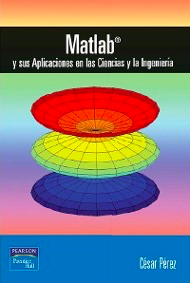
\includegraphics[scale=0.5]{images/biblio2.png}
\end{center}
\end{column}
\end{columns}
\end{frame}

\end{document}
